\documentclass[table,12pt]{article}
\usepackage[margin=1in]{geometry}
\usepackage{graphicx, float, amsmath, amssymb, multicol}

\title{\textbf{EECS 599 Project Proposal:} \\
    Comparison of Human and Simulated Reaching Movements Using Trajectory Optimization with Signal-Dependent Motor Noise}

\author{Riley Bridges and Ethan Parham \\\\
    Sensory Synapse Squad}
\date{February 2024}

\begin{document}

\maketitle
\newpage

\section{Team Charter}
\subsection{Biographies}
\begin{itemize}
    \item \begin{figure}[H]
        \centering
        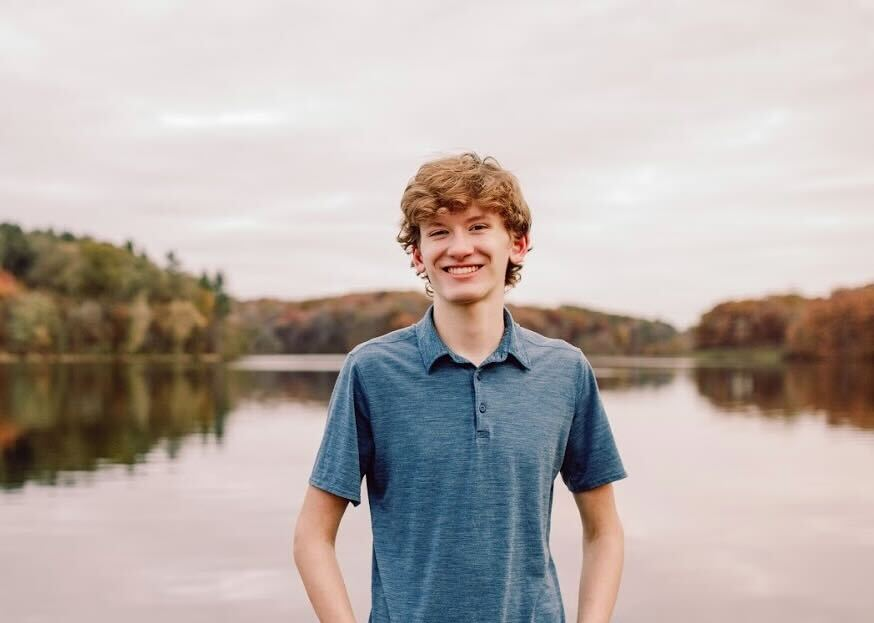
\includegraphics[width=0.3\textwidth]{riley_picture.jpg}
    \end{figure}
    \textbf{Riley Bridges:} I am a masters student at the University of Michigan studying Electrical and Computer Engineering. My main background and interest is in computer science and robotics. I love most activities involving nature, especially hiking, cycling, running, and exploration.

    \item \begin{figure}[H]
        \centering
        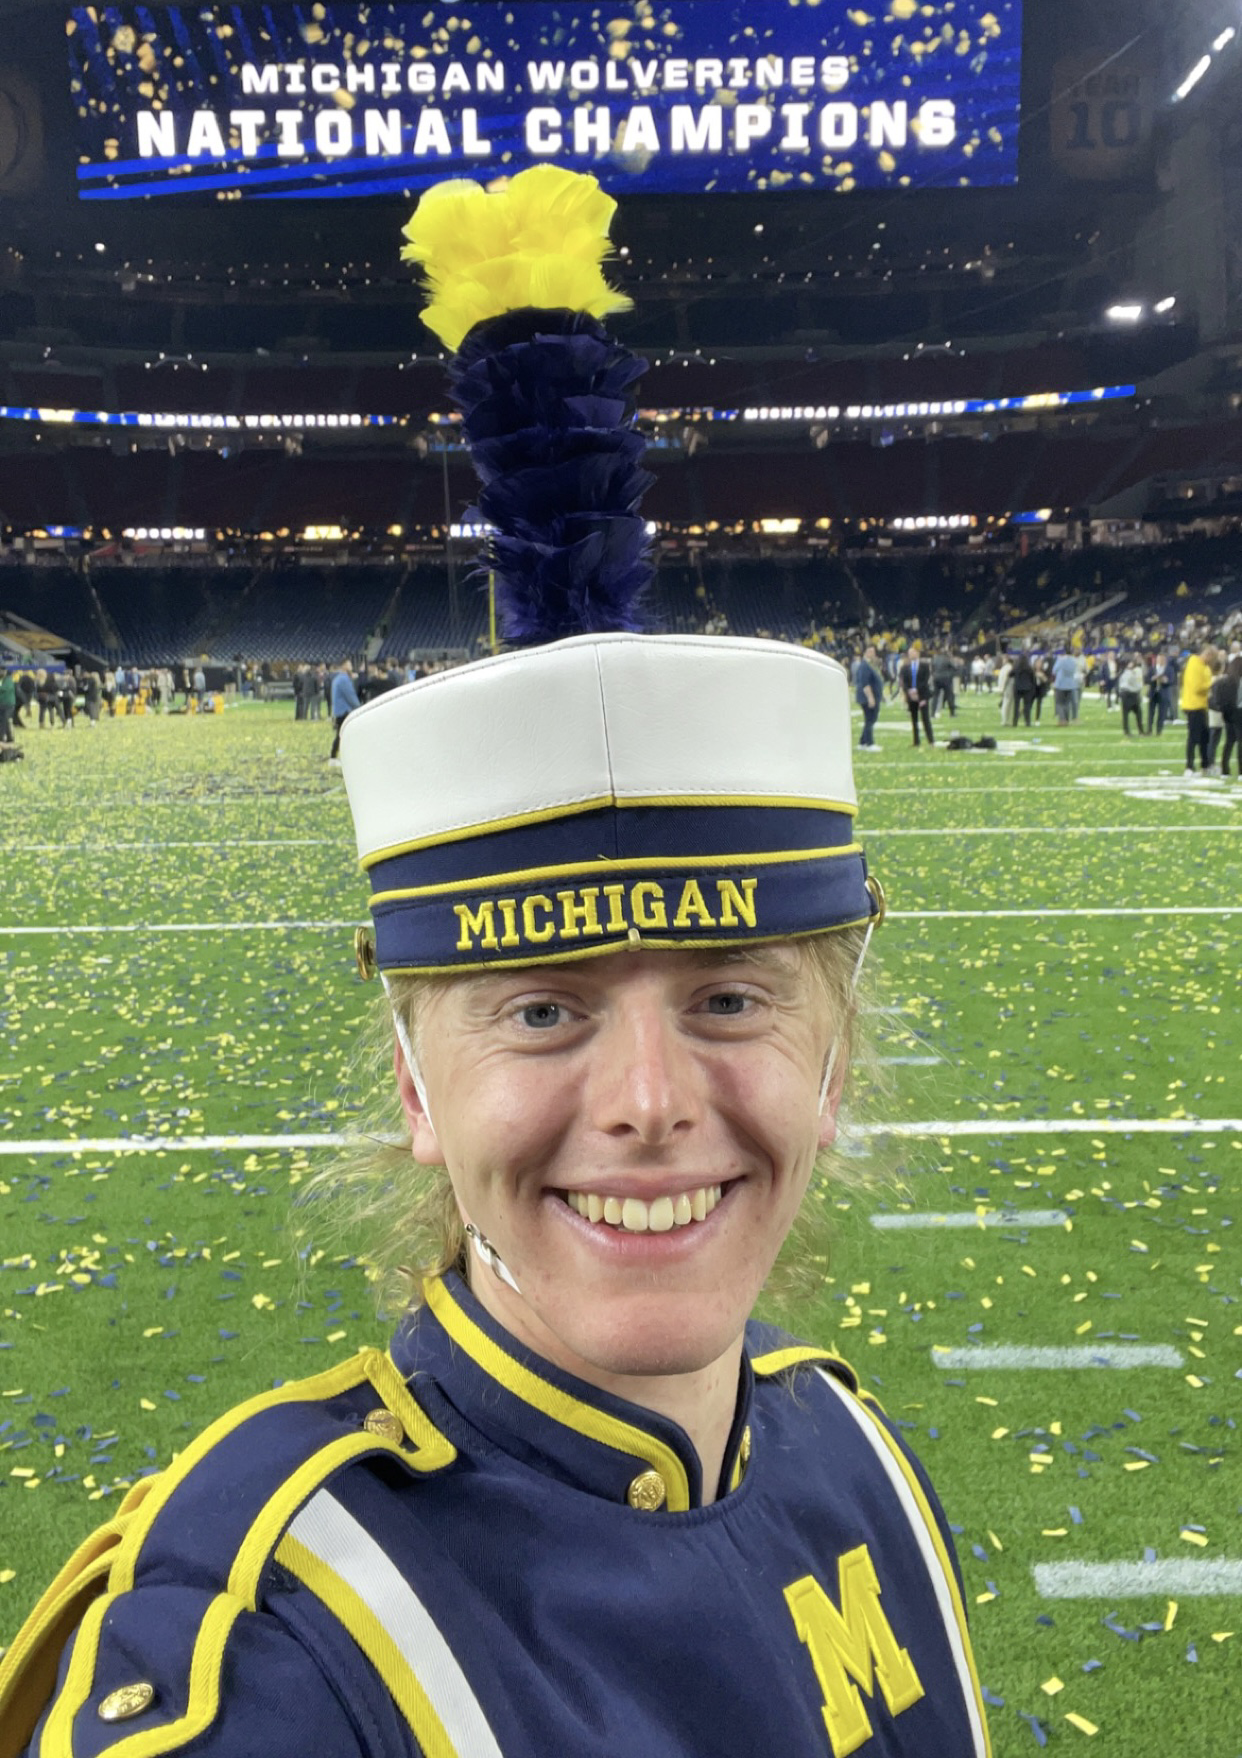
\includegraphics[width=0.3\textwidth]{ethan_picture.png}
    \end{figure}
    \textbf{Ethan Parham:} I am a graduate student at the University of Michigan studying Mechanical Engineering, concentrating on design and controls. I have a Bachelor's degree in Mechanical Engineering, with a minor in Computer Science. After I graduate, my dream role would be on a team developing prosthetics, but I also am interested in the automotive industry and environmental sustainability. One of my favorite hobbies is music, and I am heavily involved with the athletic bands at Michigan. I play trumpet in the Michigan Marching band and Hockey Band, in addition to the trumpet ensemble. 
\end{itemize}

\subsection{Vision Statement}
The members of the team aim to be able to apply controls techniques we learned in our undergraduate classes to the field of sensorimotor control. We want to be able to adapt and understand the work of other researchers, while also being able to enhance their models and control systems with our own meaningful contributions. By the end of the project, we should have a better understanding of control systems and the biological elements which relate to them, and be able to work more efficiently in a multidisciplinary field. As a result, we will be able to apply our skills to future projects even if they do not directly related to biological control.

\subsection{Responsibilities}
Each team member is expected to do an equal share of the work over the course of the project. Work will be divided according to the strengths of the team members, but the expectation is that each team member will have a good understanding of all aspects of the project and will be able to provide input to the other team members as needed. All team members should do their best to meet internal deadlines to the best of their ability. If they are unable to do so, they should notify other team members as quickly as possible so alternative plans can be made. 

\subsection{Communication Plan}
The team will communicate primarily over text when outside of meetings or class. Communication should be frequent, as it is important for all team members to be on the same page about their progress and any questions or concerns they may have. Any questions or concerns should be addressed as soon as possible, in order to maximize the working efficiency of all team members.

\subsection{Conflict Resolution}
Conflicts about content or procedure will be resolved through discussion within the group. If no resolution can be found, or the issue is more serious, then the group will propose issue to the professor for feedback or advice from a third party since as the group is a partnership no majority vote can be made. Hopefully, this feedback will allow the team to resolve their conflict.


\subsection{Meeting Plan}
The team will at minimum meet from 3-4 on Fridays on zoom. Additional or longer meetings can be scheduled as necessary. An alternative weekly meeting time is from 12-1 on Thursdays. The primary goal of the weekly meetings will be to ensure all team members are on the same page, and to set goals to be accomplished prior to the next meeting. If a team member is unable to attend the meeting, they should let the team know as soon as possible in order to reschedule to the meeting or to learn the contents of the meeting if no meeting can be made possible.

\section{Introduction and Motivation}

The speed-accuracy tradeoff is a phenomena in motor neuroscience which describes the relationship between the speed of the motion and the accuracy required of the task being performed. The tradeoff is fairly ubiquitous across different animal species as well as motor, perceptual, and cognitive tasks. As a result, understanding the relationship is a frequent topic of study, as the tradeoff must be considered in order to produce accurate models of a controlled motion \cite{c3}. The tradeoff can be quantitatively modeled using Fitts’ law.. Fitts’ Law relates the width of the target of motion $W$, the movement distance $A$, and the movement duration $MD$, as shown below \cite{c1}. Fitts law is frequently used in combination with empirical data from laboratory testing to determine the efficacy of models in relation to the speed accuracy tradeoff.  

\begin{equation}
    MD = a + b \log_2 \left(\frac{2A}{W}\right) \label{eq:fitts_law}
\end{equation}

 Historically, the speed accuracy tradeoff has been attributed to signal dependent motor noise, which is noise which has increasing variance depending on the strength of a neural control signal \cite{c2}. Noise in neural control will cause a change in the desired trajectory of a motion. These perturbations will eventually result in inaccuracies in the final movement. If noise was not a factor in the control of motion, then theoretically faster movements would result in less motor inaccuracy since there would be less time for noise to make an impact on the motion. In fact, the opposite is true as shown by Fitts’ law. The conclusion therefore is that higher speeds result in larger noise signals in motor control, resulting in larger movement variability.

 However, a new development proposes that a biomechanically realistic computational model can demonstrate the speed accuracy tradeoff without incorporating motor noise \cite{c5}. The findings propose that the speed accuracy tradeoff is caused by tighter constraints in trajectory optimization for an accurate problem which reduces the number of fast solutions for the problem. As a result, motor planning variability is the root cause of the speed accuracy tradeoff and not the motor noise as previously proposed. In order to reach this conclusion, the researchers employed a three dimensional, five degree-of-freedom model of the arm utilizing 47 muscles to produce realistic motions. Then, they utilized minimization of a cost function to model point to point movements in order to synthesize movement. They found that the motor variability can be explained using optimal control theory. Essentially, when a movement is being planned, if there is a large target there are many potential optimal paths which are found using the stochastic optimizer. Since there are more potential solutions to the movement problem, there will be many “good” solutions. However, if the search space is decreased by increasing the required accuracy needed for the movement, there will be fewer “good” options, and a less efficient option is more likely to be found when compared to a movement with lower required accuracy. Their hypothesis about motor planning was further reinforced using a study of the motor cortex of a Rhesus monkey by correlating data for the preparatory neural state variability for accurate and inaccurate tasks to the movement variability. This further emphasizes that motor planning variability results in variability in the executed motion, and indicates some kind of optimal control is involved in motor planning.

A key emphasis of the researchers is the further room for improvement on their model. Signal dependent noise and motor planning optimization are likely both contributors to the speed accuracy tradeoff as they both are able to correlate to Fitts’ law, so a model which combines both would be an improvement over either model on its own. Additionally, improvement on the optimizer used would also have potential to increase the accuracy of the model \cite{c4}.

The methods humans and animals use to optimize their motions is of great interest beyond just better modeling the reaching of a human arm. Humans are capable of performing and optimizing very complex tasks, which is a capability which is highly desirable in robotics \cite{c6}. Better understanding the speed accuracy tradeoff and the methods which are used to reduce redundancy in motion will help further the abilities of robots to perform difficult and complex tasks.

\section{Problem Description}
We aim to answer the following questions: 
\begin{itemize}
    \item When using trajectory optimization to simulate reaching movements on a human arm model, how well does the simulated behavior match human behavior, particularly with respect to the speed-accuracy tradeoff? (Question studied in \cite{c5})

    \item How does the introduction of signal-dependent motor noise to the model affect this comparison?

    \item How does the use of different trajectory optimization methods affect this comparison?
\end{itemize}
For each of these questions, we will use the following metrics to compare the simulated behavior to human behavior:
\begin{itemize}
    \item Similarity of hand velocity profile during center-out fast reaching movements, evaluated qualitatively by appearance and quantitatively by time and value of maximum velocity:
    \begin{align}
        \delta_{V_{\text{max}}} &= \max \left|V_{\text{sim}}(t)\right| - \max \left|V_{\text{exp}}(t)\right| \\
        \delta_{T_{\text{max}}} &= \arg\max_{t \in [0, t_f]} \left|V_{\text{sim}}(t)\right| - \arg\max_{t \in [0, T_f]} \left|V_{\text{exp}}(t)\right|
    \end{align}
    Where $V_{\text{sim}}$ is the simulated velocity of the hand during its reaching trajectory, $V_{\text{exp}}$ is the experimentally measured velocity of the hand during its reaching trajectory, and $t_f$ is the time at which the hand reaches the target.

    \item Delay in time of maximum velocity between large and small targets:
    \begin{multline*}
        \delta_{\text{delay}} = \left(\arg\max_{t \in [0, t_f]} \left|V_{\text{sim}}^{\text{large}}(t)\right| - \arg\max_{t \in [0, T_f]} \left|V_{\text{sim}}^{\text{small}}(t)\right|\right) \\
        - \left(\arg\max_{t \in [0, t_f]} \left|V_{\text{exp}}^{\text{large}}(t)\right| - \arg\max_{t \in [0, T_f]} \left|V_{\text{exp}}^{\text{small}}(t)\right|\right)
    \end{multline*}
    Where $V_{\text{sim}}^{\text{large}}$ and $V_{\text{sim}}^{\text{small}}$ are the simulated velocities of the hand during its reaching trajectory to large and small targets, respectively. $V_{\text{exp}}^{\text{large}}$ and $V_{\text{exp}}^{\text{small}}$ are defined similarly.
    \item Fitts' Law model parameters $a$ and $b$ (from Eq. \ref{eq:fitts_law}). 
    Several reaching tasks with fixed target distance and variable target width will be simulated. A least squares regression will then be used on movement duration $MD$ and target width $W$ data for each trial in order to fit the parameters:
    \begin{align}
        \begin{bmatrix}
            a^* \\ b^*
        \end{bmatrix} &= \arg\min_{a, b} \sum_{i=1}^N \left(MD_i - \left(a + b \log_2\left(\frac{2A}{W_i}\right)\right)\right)^2
    \end{align}
    Where $MD_i$ and $W_i$ are the movement duration and target width, respectively, for the $i$th trial, and $N$ is the number of trials.
\end{itemize}

We will formulate our signal-dependent motor noise (roughly) as additive gaussian noise proportional to the control input for each actuator:
\begin{align}
    \tilde{u}_i(t) = u_i(t) + u_i(t) \cdot w_i(t), \quad w_i(t) \sim \mathcal{N}(0, \sigma_i^2)
\end{align}
This formulation is subject to change based on further literature review.

While we intend to experiment with different trajectory optimization methods, they will all roughly fall into the following general optimization problem:
\begin{align}
    \arg\min_{\mathbf{u}(t)} &\quad G\left(\mathbf{x}(t_f), t_f\right) + \int_0^{t_f} E(\mathbf{x}(t), \mathbf{u}(t)) dt \\
    \text{subject to} &\quad \dot{\mathbf{x}}(t) = f(\mathbf{x}(t), \mathbf{u}(t)), \quad \mathbf{x}(0) = \mathbf{x}_0 \\
    &\quad C(\mathbf{x}(t_f)) \leq \mathbf{0}
\end{align}
Where $\mathbf{x}(t)$ is the state of the system at time $t$, $\mathbf{u}(t)$ is the control input at time $t$, $G$ is some cost function associated with the final state and time, $E$ is some cost function representing the energy cost of a given state and control input, $f$ is the dynamics of the system, $\mathbf{x}_0$ is the initial state of the system, and $C$ is some constraint function associated with the final state.

Different methods may use different cost functions and constraints, and several different methods for solving the optimization problem will be used. Some of these may include: constrained single shooting, multiple shooting, and direct collocation. It should also be mentioned that the above dynamics and optimization problem will be discretized for numerical computation.

\subsection{System Model and Stochastic Dynamics}
Our human arm system is modeled as a 2 degree of freedom planar arm with shoulder and elbow joints, actuated by 6 Hill-type muscles. This model has been adapted from the model used in TODO. The state and control input vectors are defined below:
TODO: add figure
\begin{align}
    \mathbf{x} &= \begin{bmatrix}
        \mathbf{q} &
        \dot{\mathbf{q}}
    \end{bmatrix}^\top = \begin{bmatrix}
        \theta_s &
        \theta_e &
        \dot{\theta}_s &
        \dot{\theta}_e
    \end{bmatrix}^\top \\
    \mathbf{u} &= \begin{bmatrix}
        a_{\text{brach}} & a_{\text{lattri}} & a_{\text{antdel}} & a_{\text{postdel}} & a_{\text{bic}} & a_{\text{lattri}}
    \end{bmatrix}
\end{align}

Where $\theta_s$ and $\theta_e$ are the shoulder and elbow joint angles, respectively, and $\dot{\theta}_s$ and $\dot{\theta}_e$ are the corresponding joint angular velocities. The control input $\mathbf{u}$ is a vector of muscle activations for each of the 6 muscles in the model. The stochastic dynamics of the system are given by the following differential equation:

\begin{align}
    \dot{\mathbf{x}} &= f(\mathbf{x}, \mathbf{u}, \mathbf{w}) \quad \mathbf{w} \sim \mathcal{N}(0, \Sigma_w) \\
    &= \begin{bmatrix}
        \dot{\mathbf{q}} \\
        M(\mathbf{q})^{-1} \left(C(\mathbf{q}, \dot{\mathbf{q}}) + T_M(\tilde{\mathbf{u}}, \mathbf{q})\right)
    \end{bmatrix} \\
    \tilde{\mathbf{u}} &= \mathbf{u} + \text{diag}(\mathbf{u}) \cdot \mathbf{w}
\end{align}

Where $M(\mathbf{q})$ is the mass matrix of the arm model, $C(\mathbf{q}, \dot{\mathbf{q}})$ is the term describing the Coriolis forces, and $T_M(\mathbf{u}, \mathbf{q})$ is the term describing the torques generated by the muscles. Further details on the dynamics of the system can be found in TODO.

\section{Planned Approach}
\subsection{Timeline}
\begin{itemize}
    \item \textbf{2/19} Riley: Setup OpenSim simulation software and development environment, evaluate feasibility of using original complex model by running simulation using code provided in the original paper.

    Ethan: Review literature relating to signal-dependent motor noise, begin developing a formulation for introducing this noise to the model/simulation.

    \item \textbf{2/26 (Spring Break)} Riley: Help with implementation of noise in simulation (dependent on completed mathematical formulation), begin literature review of trajectory optimization methods applicable to high dimensional arm models.

    Ethan: Finish formulation of motor noise in simulation model, implement noise in simulation by modifying original C++ code.

    \item \textbf{3/4} Riley: Develop scripts to evaluate metrics on collected simulation data, test and iterate on the noise implementation (dependent on completed initial implementation).

    Ethan: Collect experimental data from previous human reaching studies, run several trials of the simulation with and without noise (dependent on completed noise implementation).

    \item \textbf{3/11 (Progress Report)} Riley: Prepare project progress report, began formulation and testing of different trajectory optimization methods in MATLAB.

    Ethan: Prepare project progress report, continue running trials of the simulation with and without noise, begin analysis of collected data.

    \item \textbf{3/18} Riley: Choose a trajectory optimization method and implement it in C++ for use in the simulation (dependent on completed formulation and testing in MATLAB), research and test different numerical optimizers available for C++.

    Ethan: Complete analysis of collected motor noise data and comparison to experimental data, review trajectory optimization methods.

    \item \textbf{3/25} Riley: Test and iterate on the trajectory optimization implementation (dependent on completed initial implementation).

    Ethan: Choose a different trajectory optimization method and begin formulating and testing it in MATLAB.

    \item \textbf{4/1} Riley: Continue testing and iterating on the trajectory optimization implementation, begin running trials and collecting data for metrics, begin preparing background slides for final presentation

    Ethan: Implement and begin testing the chosen trajectory optimization method in C++. (dependent on completed formulation and testing in MATLAB), begin preparing background slides for final presentation.

    \item \textbf{4/8} Riley: Continue running trials and collecting data for metrics, begin analysis of collected data, continue preparing slides for final presentation.

    Ethan: Continue testing and iterating on the trajectory optimization implementation, begin running trials and collecting data for metrics, continue preparing slides for final presentation.

    \item \textbf{4/15} Riley: Finish analysis of collected data, finish final presentation, begin final report.

    Ethan: Finish running trials and collecting data for metrics, finish final presentation, begin final report.

    \item \textbf{4/22 (Final Report)} Riley: Finish final report.

    Ethan: Finish final report.

\end{itemize}
\subsection{Anticipated Challenges}
One of the main challenges we anticipate to complexity of the model we intend to use for simulation. This model is a high fidelity biologically accurate model of the human arm including 47 muscle-tendon actuators and 5 degrees of freedom. This complexity may cause our optimal control simulations to be prohibitively slow to run, and it may make it difficult to implement the signal-dependent motor noise. If we encounter these problems, we plan to instead use a simplified human arm model with fewer actuators. This may reduce our ability to accurately replicate human behavior, but it will allow us to complete the project in a reasonable amount of time.

Another challenge we anticipate is use of the OpenSim simulation software and C++ programming language. Neither of us have experience using OpenSim, so it is possible that there will be very significant learning curve to overcome, or even that it will lack features we need in order to complete the project. Although we both have experience using C++, we have never used it for optimal control. Because this use case often requires well developed libraries and optimization tools (e.g. fmincon in MATLAB) in order for rapid prototyping and testing to be feasible, we may encounter significant difficulty in implementing our optimal control simulations in C++ if these tools and libraries are not available. If we encounter these problems, we plan to use MATLAB instead of C++ for the optimal control simulations. MATLAB is known to have a well developed set of tools for use with trajectory optimization, and one of us has direct experience using it for that purpose. If this prevents us from using the original complex model, we will use a simplified model as described above.

\section{Goals and Evaluation}
As a baseline goal for this project, we aim to modify the simulation and control method from the original paper to include signal-dependent motor noise and produce a meaningful comparison between the these new simulated results and experimental data collected from previous studies. Specifically, we will consider this project successful if we are able to do the following:
\begin{itemize}
    \item Incorporate motor noise into our simulation in a way that is, at least in some aspects, biologically realistic and backed up by previous literature.
    \item Run this simulation and collect data from a sufficient number of trials (at least 10) for each reaching task described in the Problem Description section.
    \item Analyze the collected data and compare it to experimental data from previous studies, using the metrics described in the Problem Description section.
\end{itemize}

As a stretch goal, we aim to compare the results of the original trajectory optimization method used in the original paper to the results of one or more alternative trajectory optimization methods. Specifically, we will consider this goal successful if we are able to do the following:
\begin{itemize}
    \item Choose one or more alternative trajectory optimization methods and implement them in our simulation.
    \item Run the simulation and collect data from a sufficient number of trials (at least 10) for each reaching task described in the Problem Description section using the alternative trajectory optimization method(s).
    \item Analyze the collected data and compare it to the original trajectory optimization method using the metrics described in the Problem Description section.
\end{itemize}

\begin{thebibliography}{99}
\bibitem{c1}
Fitts PM (1954) The information capacity of the human motor system in controlling the amplitude of movement Journal of Experimental Psychology 47:381–391. https://doi.org/10.1037/h0055392 

\bibitem{c2}
Harris, C., Wolpert, D. Signal-dependent noise determines motor planning. Nature 394, 780–784 (1998). https://doi.org/10.1038/29528

\bibitem{c3}
Heitz RP (2014) The speed-accuracy tradeoff: history, physiology, methodology, and behavior Frontiers in Neuroscience 8:150. https://doi.org/10.3389/fnins.2014.00150

\bibitem{c4}
Lillicrap TP, Hunt JJ, Pritzel A, Heess N, Erez T, Tassa Y, Silver D, Wierstra D (2015) Continuous control with deep reinforcement learning arXiv. https://arxiv.org/abs/1509.02971

\bibitem{c5}
Mazen Al Borno, Saurabh Vyas, Krishna V Shenoy, Scott L Delp (2020) High-fidelity musculoskeletal modeling reveals that motor planning variability contributes to the speed-accuracy tradeoff 
https://doi.org/eLife 9:e57021

\bibitem{c6}
Trivedi U, Menychtas D, Alqasemi R, Dubey R. Biomimetic Approaches for Human Arm Motion Generation: Literature Review and Future Directions. Sensors (Basel). 2023 Apr 12;23(8):3912. doi: 10.3390/s23083912.
\end{thebibliography}
\end{document}
\documentclass[table,12pt]{article}
\usepackage[margin=1in]{geometry}
\usepackage{graphicx, float, amsmath, amssymb, multicol}

\title{\textbf{EECS 599 Project Proposal:} \\
    Comparison of Human and Simulated Reaching Movements Using Trajectory Optimization with Signal-Dependent Motor Noise}

\author{Riley Bridges and Ethan Parham \\\\
    Sensory Synapse Squad}
\date{February 2024}

\begin{document}

\maketitle
\newpage

\section{Team Charter}
\subsection{Biographies}
\begin{itemize}
    \item \begin{figure}[H]
        \centering
        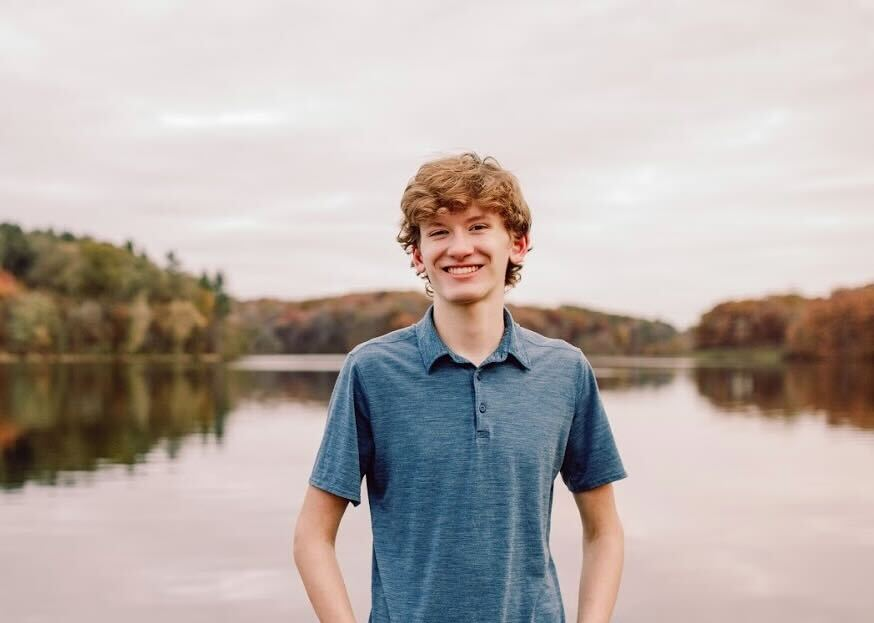
\includegraphics[width=0.3\textwidth]{riley_picture.jpg}
    \end{figure}
    \textbf{Riley Bridges:} I am a masters student at the University of Michigan studying Electrical and Computer Engineering. My main background and interest is in computer science and robotics. I love most activities involving nature, especially hiking, cycling, running, and exploration.

    \item \begin{figure}[H]
        \centering
        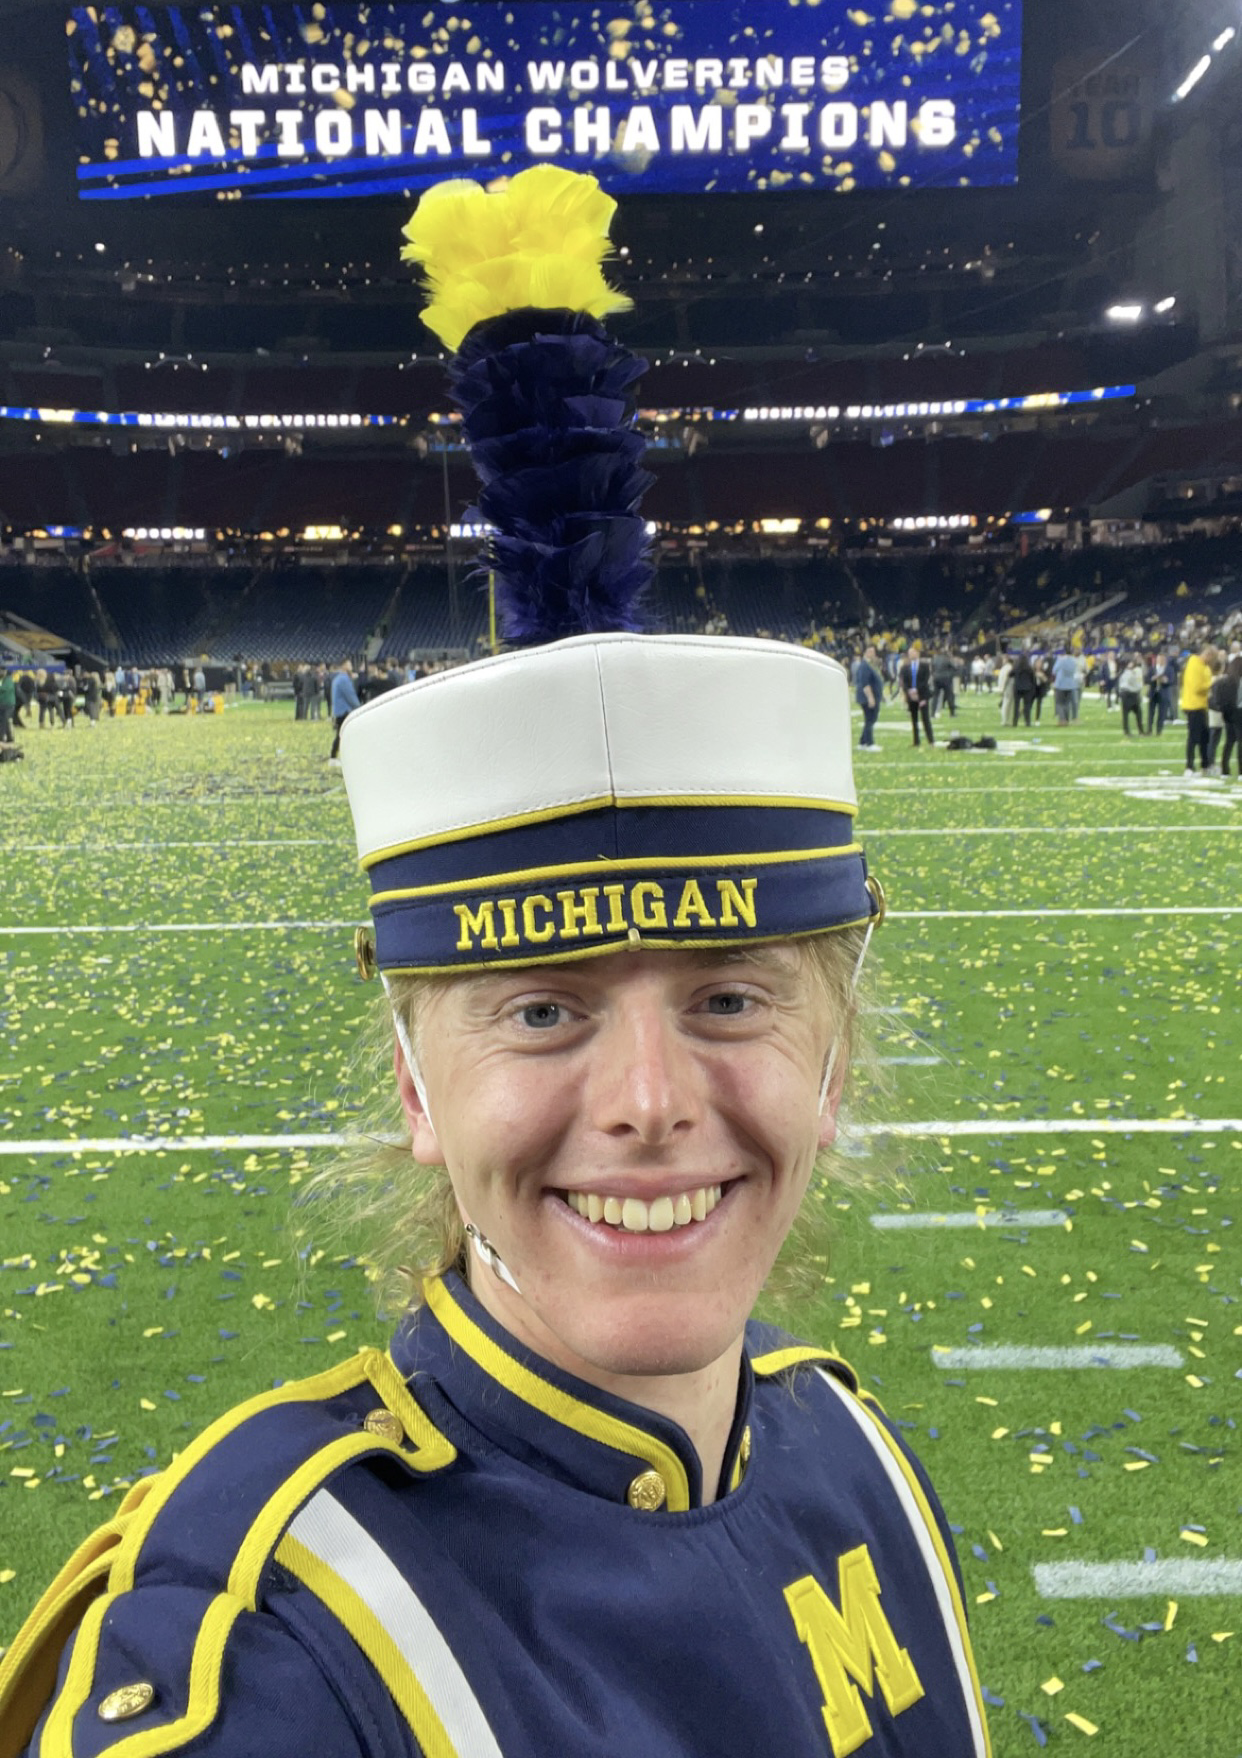
\includegraphics[width=0.3\textwidth]{ethan_picture.png}
    \end{figure}
    \textbf{Ethan Parham:} I am a graduate student at the University of Michigan studying Mechanical Engineering, concentrating on design and controls. I have a Bachelor's degree in Mechanical Engineering, with a minor in Computer Science. After I graduate, my dream role would be on a team developing prosthetics, but I also am interested in the automotive industry and environmental sustainability. One of my favorite hobbies is music, and I am heavily involved with the athletic bands at Michigan. I play trumpet in the Michigan Marching band and Hockey Band, in addition to the trumpet ensemble. 
\end{itemize}

\subsection{Vision Statement}
The members of the team aim to be able to apply controls techniques we learned in our undergraduate classes to the field of sensorimotor control. We want to be able to adapt and understand the work of other researchers, while also being able to enhance their models and control systems with our own meaningful contributions. By the end of the project, we should have a better understanding of control systems and the biological elements which relate to them, and be able to work more efficiently in a multidisciplinary field. As a result, we will be able to apply our skills to future projects even if they do not directly related to biological control.

\subsection{Responsibilities}
Each team member is expected to do an equal share of the work over the course of the project. Work will be divided according to the strengths of the team members, but the expectation is that each team member will have a good understanding of all aspects of the project and will be able to provide input to the other team members as needed. All team members should do their best to meet internal deadlines to the best of their ability. If they are unable to do so, they should notify other team members as quickly as possible so alternative plans can be made. 

\subsection{Communication Plan}
The team will communicate primarily over text when outside of meetings or class. Communication should be frequent, as it is important for all team members to be on the same page about their progress and any questions or concerns they may have. Any questions or concerns should be addressed as soon as possible, in order to maximize the working efficiency of all team members.

\subsection{Conflict Resolution}
Conflicts about content or procedure will be resolved through discussion within the group. If no resolution can be found, or the issue is more serious, then the group will propose issue to the professor for feedback or advice from a third party since as the group is a partnership no majority vote can be made. Hopefully, this feedback will allow the team to resolve their conflict.


\subsection{Meeting Plan}
The team will at minimum meet from 3-4 on Fridays on zoom. Additional or longer meetings can be scheduled as necessary. An alternative weekly meeting time is from 12-1 on Thursdays. The primary goal of the weekly meetings will be to ensure all team members are on the same page, and to set goals to be accomplished prior to the next meeting. If a team member is unable to attend the meeting, they should let the team know as soon as possible in order to reschedule to the meeting or to learn the contents of the meeting if no meeting can be made possible.

\section{Introduction and Motivation}

The speed-accuracy tradeoff is a phenomena in motor neuroscience which describes the relationship between the speed of the motion and the accuracy required of the task being performed. The tradeoff is fairly ubiquitous across different animal species as well as motor, perceptual, and cognitive tasks. As a result, understanding the relationship is a frequent topic of study, as the tradeoff must be considered in order to produce accurate models of a controlled motion \cite{c3}. The tradeoff can be quantitatively modeled using Fitts’ law.. Fitts’ Law relates the width of the target of motion $W$, the movement distance $A$, and the movement duration $MD$, as shown below \cite{c1}. Fitts law is frequently used in combination with empirical data from laboratory testing to determine the efficacy of models in relation to the speed accuracy tradeoff.  

\begin{equation}
    MD = a + b \log_2 \left(\frac{2A}{W}\right) \label{eq:fitts_law}
\end{equation}

 Historically, the speed accuracy tradeoff has been attributed to signal dependent motor noise, which is noise which has increasing variance depending on the strength of a neural control signal \cite{c2}. Noise in neural control will cause a change in the desired trajectory of a motion. These perturbations will eventually result in inaccuracies in the final movement. If noise was not a factor in the control of motion, then theoretically faster movements would result in less motor inaccuracy since there would be less time for noise to make an impact on the motion. In fact, the opposite is true as shown by Fitts’ law. The conclusion therefore is that higher speeds result in larger noise signals in motor control, resulting in larger movement variability.

 However, a new development proposes that a biomechanically realistic computational model can demonstrate the speed accuracy tradeoff without incorporating motor noise \cite{c5}. The findings propose that the speed accuracy tradeoff is caused by tighter constraints in trajectory optimization for an accurate problem which reduces the number of fast solutions for the problem. As a result, motor planning variability is the root cause of the speed accuracy tradeoff and not the motor noise as previously proposed. In order to reach this conclusion, the researchers employed a three dimensional, five degree-of-freedom model of the arm utilizing 47 muscles to produce realistic motions. Then, they utilized minimization of a cost function to model point to point movements in order to synthesize movement. They found that the motor variability can be explained using optimal control theory. Essentially, when a movement is being planned, if there is a large target there are many potential optimal paths which are found using the stochastic optimizer. Since there are more potential solutions to the movement problem, there will be many “good” solutions. However, if the search space is decreased by increasing the required accuracy needed for the movement, there will be fewer “good” options, and a less efficient option is more likely to be found when compared to a movement with lower required accuracy. Their hypothesis about motor planning was further reinforced using a study of the motor cortex of a Rhesus monkey by correlating data for the preparatory neural state variability for accurate and inaccurate tasks to the movement variability. This further emphasizes that motor planning variability results in variability in the executed motion, and indicates some kind of optimal control is involved in motor planning.

A key emphasis of the researchers is the further room for improvement on their model. Signal dependent noise and motor planning optimization are likely both contributors to the speed accuracy tradeoff as they both are able to correlate to Fitts’ law, so a model which combines both would be an improvement over either model on its own. Additionally, improvement on the optimizer used would also have potential to increase the accuracy of the model \cite{c4}.

The methods humans and animals use to optimize their motions is of great interest beyond just better modeling the reaching of a human arm. Humans are capable of performing and optimizing very complex tasks, which is a capability which is highly desirable in robotics \cite{c6}. Better understanding the speed accuracy tradeoff and the methods which are used to reduce redundancy in motion will help further the abilities of robots to perform difficult and complex tasks.

\section{Problem Description}
We aim to answer the following questions: 
\begin{itemize}
    \item When using trajectory optimization to simulate reaching movements on a human arm model, how well does the simulated behavior match human behavior, particularly with respect to the speed-accuracy tradeoff? (Question studied in \cite{c5})

    \item How does the introduction of signal-dependent motor noise to the model affect this comparison?

    \item How does the use of different trajectory optimization methods affect this comparison?
\end{itemize}
For each of these questions, we will use the following metrics to compare the simulated behavior to human behavior:
\begin{itemize}
    \item Similarity of hand velocity profile during center-out fast reaching movements, evaluated qualitatively by appearance and quantitatively by time and value of maximum velocity:
    \begin{align}
        \delta_{V_{\text{max}}} &= \max \left|V_{\text{sim}}(t)\right| - \max \left|V_{\text{exp}}(t)\right| \\
        \delta_{T_{\text{max}}} &= \arg\max_{t \in [0, t_f]} \left|V_{\text{sim}}(t)\right| - \arg\max_{t \in [0, T_f]} \left|V_{\text{exp}}(t)\right|
    \end{align}
    Where $V_{\text{sim}}$ is the simulated velocity of the hand during its reaching trajectory, $V_{\text{exp}}$ is the experimentally measured velocity of the hand during its reaching trajectory, and $t_f$ is the time at which the hand reaches the target.

    \item Delay in time of maximum velocity between large and small targets:
    \begin{multline*}
        \delta_{\text{delay}} = \left(\arg\max_{t \in [0, t_f]} \left|V_{\text{sim}}^{\text{large}}(t)\right| - \arg\max_{t \in [0, T_f]} \left|V_{\text{sim}}^{\text{small}}(t)\right|\right) \\
        - \left(\arg\max_{t \in [0, t_f]} \left|V_{\text{exp}}^{\text{large}}(t)\right| - \arg\max_{t \in [0, T_f]} \left|V_{\text{exp}}^{\text{small}}(t)\right|\right)
    \end{multline*}
    Where $V_{\text{sim}}^{\text{large}}$ and $V_{\text{sim}}^{\text{small}}$ are the simulated velocities of the hand during its reaching trajectory to large and small targets, respectively. $V_{\text{exp}}^{\text{large}}$ and $V_{\text{exp}}^{\text{small}}$ are defined similarly.
    \item Fitts' Law model parameters $a$ and $b$ (from Eq. \ref{eq:fitts_law}). 
    Several reaching tasks with fixed target distance and variable target width will be simulated. A least squares regression will then be used on movement duration $MD$ and target width $W$ data for each trial in order to fit the parameters:
    \begin{align}
        \begin{bmatrix}
            a^* \\ b^*
        \end{bmatrix} &= \arg\min_{a, b} \sum_{i=1}^N \left(MD_i - \left(a + b \log_2\left(\frac{2A}{W_i}\right)\right)\right)^2
    \end{align}
    Where $MD_i$ and $W_i$ are the movement duration and target width, respectively, for the $i$th trial, and $N$ is the number of trials.
\end{itemize}

We will formulate our signal-dependent motor noise (roughly) as additive gaussian noise proportional to the control input for each actuator:
\begin{align}
    \tilde{u}_i(t) = u_i(t) + u_i(t) \cdot w_i(t), \quad w_i(t) \sim \mathcal{N}(0, \sigma_i^2)
\end{align}
This formulation is subject to change based on further literature review.

While we intend to experiment with different trajectory optimization methods, they will all roughly fall into the following general optimization problem:
\begin{align}
    \arg\min_{\mathbf{u}(t)} &\quad G\left(\mathbf{x}(t_f), t_f\right) + \int_0^{t_f} E(\mathbf{x}(t), \mathbf{u}(t)) dt \\
    \text{subject to} &\quad \dot{\mathbf{x}}(t) = f(\mathbf{x}(t), \mathbf{u}(t)), \quad \mathbf{x}(0) = \mathbf{x}_0 \\
    &\quad C(\mathbf{x}(t_f)) \leq \mathbf{0}
\end{align}
Where $\mathbf{x}(t)$ is the state of the system at time $t$, $\mathbf{u}(t)$ is the control input at time $t$, $G$ is some cost function associated with the final state and time, $E$ is some cost function representing the energy cost of a given state and control input, $f$ is the dynamics of the system, $\mathbf{x}_0$ is the initial state of the system, and $C$ is some constraint function associated with the final state.

Different methods may use different cost functions and constraints, and several different methods for solving the optimization problem will be used. Some of these may include: constrained single shooting, multiple shooting, and direct collocation. It should also be mentioned that the above dynamics and optimization problem will be discretized for numerical computation.

\section{Planned Approach}
\subsection{Timeline}
\begin{itemize}
    \item \textbf{2/19} Riley: Setup OpenSim simulation software and development environment, evaluate feasibility of using original complex model by running simulation using code provided in the original paper.

    Ethan: Review literature relating to signal-dependent motor noise, begin developing a formulation for introducing this noise to the model/simulation.

    \item \textbf{2/26 (Spring Break)} Riley: Help with implementation of noise in simulation (dependent on completed mathematical formulation), begin literature review of trajectory optimization methods applicable to high dimensional arm models.

    Ethan: Finish formulation of motor noise in simulation model, implement noise in simulation by modifying original C++ code.

    \item \textbf{3/4} Riley: Develop scripts to evaluate metrics on collected simulation data, test and iterate on the noise implementation (dependent on completed initial implementation).

    Ethan: Collect experimental data from previous human reaching studies, run several trials of the simulation with and without noise (dependent on completed noise implementation).

    \item \textbf{3/11 (Progress Report)} Riley: Prepare project progress report, began formulation and testing of different trajectory optimization methods in MATLAB.

    Ethan: Prepare project progress report, continue running trials of the simulation with and without noise, begin analysis of collected data.

    \item \textbf{3/18} Riley: Choose a trajectory optimization method and implement it in C++ for use in the simulation (dependent on completed formulation and testing in MATLAB), research and test different numerical optimizers available for C++.

    Ethan: Complete analysis of collected motor noise data and comparison to experimental data, review trajectory optimization methods.

    \item \textbf{3/25} Riley: Test and iterate on the trajectory optimization implementation (dependent on completed initial implementation).

    Ethan: Choose a different trajectory optimization method and begin formulating and testing it in MATLAB.

    \item \textbf{4/1} Riley: Continue testing and iterating on the trajectory optimization implementation, begin running trials and collecting data for metrics, begin preparing background slides for final presentation

    Ethan: Implement and begin testing the chosen trajectory optimization method in C++. (dependent on completed formulation and testing in MATLAB), begin preparing background slides for final presentation.

    \item \textbf{4/8} Riley: Continue running trials and collecting data for metrics, begin analysis of collected data, continue preparing slides for final presentation.

    Ethan: Continue testing and iterating on the trajectory optimization implementation, begin running trials and collecting data for metrics, continue preparing slides for final presentation.

    \item \textbf{4/15} Riley: Finish analysis of collected data, finish final presentation, begin final report.

    Ethan: Finish running trials and collecting data for metrics, finish final presentation, begin final report.

    \item \textbf{4/22 (Final Report)} Riley: Finish final report.

    Ethan: Finish final report.

\end{itemize}
\subsection{Anticipated Challenges}
One of the main challenges we anticipate to complexity of the model we intend to use for simulation. This model is a high fidelity biologically accurate model of the human arm including 47 muscle-tendon actuators and 5 degrees of freedom. This complexity may cause our optimal control simulations to be prohibitively slow to run, and it may make it difficult to implement the signal-dependent motor noise. If we encounter these problems, we plan to instead use a simplified human arm model with fewer actuators. This may reduce our ability to accurately replicate human behavior, but it will allow us to complete the project in a reasonable amount of time.

Another challenge we anticipate is use of the OpenSim simulation software and C++ programming language. Neither of us have experience using OpenSim, so it is possible that there will be very significant learning curve to overcome, or even that it will lack features we need in order to complete the project. Although we both have experience using C++, we have never used it for optimal control. Because this use case often requires well developed libraries and optimization tools (e.g. fmincon in MATLAB) in order for rapid prototyping and testing to be feasible, we may encounter significant difficulty in implementing our optimal control simulations in C++ if these tools and libraries are not available. If we encounter these problems, we plan to use MATLAB instead of C++ for the optimal control simulations. MATLAB is known to have a well developed set of tools for use with trajectory optimization, and one of us has direct experience using it for that purpose. If this prevents us from using the original complex model, we will use a simplified model as described above.

\section{Goals and Evaluation}
As a baseline goal for this project, we aim to modify the simulation and control method from the original paper to include signal-dependent motor noise and produce a meaningful comparison between the these new simulated results and experimental data collected from previous studies. Specifically, we will consider this project successful if we are able to do the following:
\begin{itemize}
    \item Incorporate motor noise into our simulation in a way that is, at least in some aspects, biologically realistic and backed up by previous literature.
    \item Run this simulation and collect data from a sufficient number of trials (at least 10) for each reaching task described in the Problem Description section.
    \item Analyze the collected data and compare it to experimental data from previous studies, using the metrics described in the Problem Description section.
\end{itemize}

As a stretch goal, we aim to compare the results of the original trajectory optimization method used in the original paper to the results of one or more alternative trajectory optimization methods. Specifically, we will consider this goal successful if we are able to do the following:
\begin{itemize}
    \item Choose one or more alternative trajectory optimization methods and implement them in our simulation.
    \item Run the simulation and collect data from a sufficient number of trials (at least 10) for each reaching task described in the Problem Description section using the alternative trajectory optimization method(s).
    \item Analyze the collected data and compare it to the original trajectory optimization method using the metrics described in the Problem Description section.
\end{itemize}

\begin{thebibliography}{99}
\bibitem{c1}
Fitts PM (1954) The information capacity of the human motor system in controlling the amplitude of movement Journal of Experimental Psychology 47:381–391. https://doi.org/10.1037/h0055392 

\bibitem{c2}
Harris, C., Wolpert, D. Signal-dependent noise determines motor planning. Nature 394, 780–784 (1998). https://doi.org/10.1038/29528

\bibitem{c3}
Heitz RP (2014) The speed-accuracy tradeoff: history, physiology, methodology, and behavior Frontiers in Neuroscience 8:150. https://doi.org/10.3389/fnins.2014.00150

\bibitem{c4}
Lillicrap TP, Hunt JJ, Pritzel A, Heess N, Erez T, Tassa Y, Silver D, Wierstra D (2015) Continuous control with deep reinforcement learning arXiv. https://arxiv.org/abs/1509.02971

\bibitem{c5}
Mazen Al Borno, Saurabh Vyas, Krishna V Shenoy, Scott L Delp (2020) High-fidelity musculoskeletal modeling reveals that motor planning variability contributes to the speed-accuracy tradeoff 
https://doi.org/eLife 9:e57021

\bibitem{c6}
Trivedi U, Menychtas D, Alqasemi R, Dubey R. Biomimetic Approaches for Human Arm Motion Generation: Literature Review and Future Directions. Sensors (Basel). 2023 Apr 12;23(8):3912. doi: 10.3390/s23083912.
\end{thebibliography}
\end{document}
